\chapter{操作系统支持}

\section{虚拟内存支持}\label{section:TLB}

\cpuname 支持了MIPS规范中基于TLB的虚拟地址转换功能。
由于MIPS指令集架构中,TLB采用全相连的结构,匹配需要大量的电路延迟,为了保证运行操作系统时的频率,我们将TLB拆为两级。

\begin{figure}[h]
    \centering
    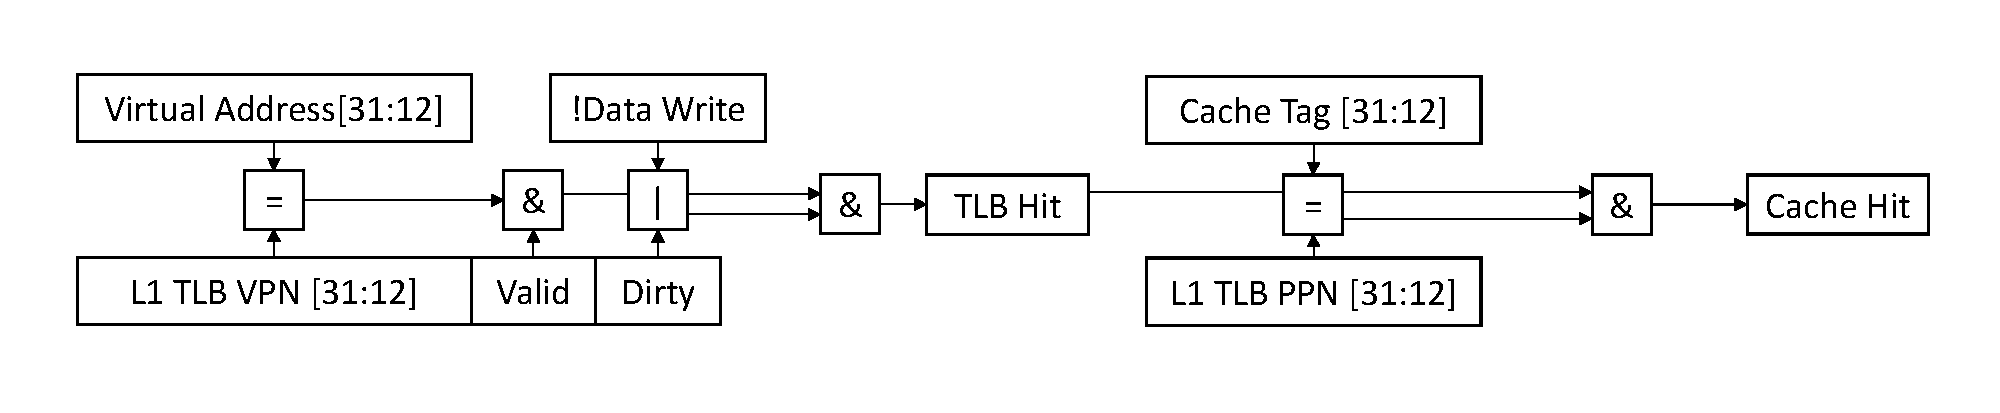
\includegraphics[width=\linewidth]{l1_tlb.pdf}
    \caption{一级TLB的设计}
    \label{img:l1_tlb}
\end{figure}

其中,一级TLB分为一级指令TLB与一级数据TLB,各只有一项,位于指令Cache与数据Cache中。
由于我们的Cache单路恰好为4KB,恰好为我们处理器支持的最小页面大小,因此采用伪VIPT(Virtually Indexed Physically Tagged)方式,比较方式如图\ref{img:l1_tlb}所示。

在我们的设计中,一级TLB与Cache状态机深度整合,且在一级TLB命中的情况下不会带来额外的流水线停顿,由此兼顾了IPC与频率。

二级TLB采用全相连结构,有8项,位于CP0中,提供了3个可同时访问的查找接口分别用于TLBP指令、一级指令TLB、一级数据TLB。
当一级TLB缺失时,会向CP0中的L2 TLB发出缺失的VPN2地址(虚拟地址的[31:27]部分)进行TLB查找,并在下一周期得到对应的TLB表项以及是否命中成功。
当出现L2 TLB查找失败、TLB无效、写只读页等情况时,则根据当前状态发出对应的异常,跳转到异常处理地址交给系统内核完成TLB的回填操作。

由于我们TLB做了两级,需要解决L1 TLB与L2 TLB间的一致性问题,这里需要考虑两种情况,一种是ASID切换,另一种是TLB写入。
我们采用的设计是在L1 TLB中添加一个清空TLB的信号,并在执行MTC0、TLBWI、TLBWR三条指令时都拉高清空信号,以解决虚拟地址重名问题。

\section{Cache指令支持}

由于操作系统中存在写入指令后执行,与DMA前后写回或失效Cache的操作,这需要Cache指令的支持。这一部分已在Cache章节有所介绍。
且经过我们测试发现Linux不会使用Index Store Tag这样特殊的Cache指令,因此这样简单的实现就满足了运行Linux的要求。

\section{U-Boot}

我们继承了前辈NSCSCC 2019 清华大学 编程是一件很危险的事情 与 NSCSCC 2021 北京航空航天大学一队的工作,为我们的CPU移植的U-Boot。
主要工作包括编写设备树、修改配置文件、修改串口时钟频率。最终我们成功运行起了U-Boot并能够通过tftp载入uCore与Linux操作系统。

\begin{figure}[h]
    \centering
    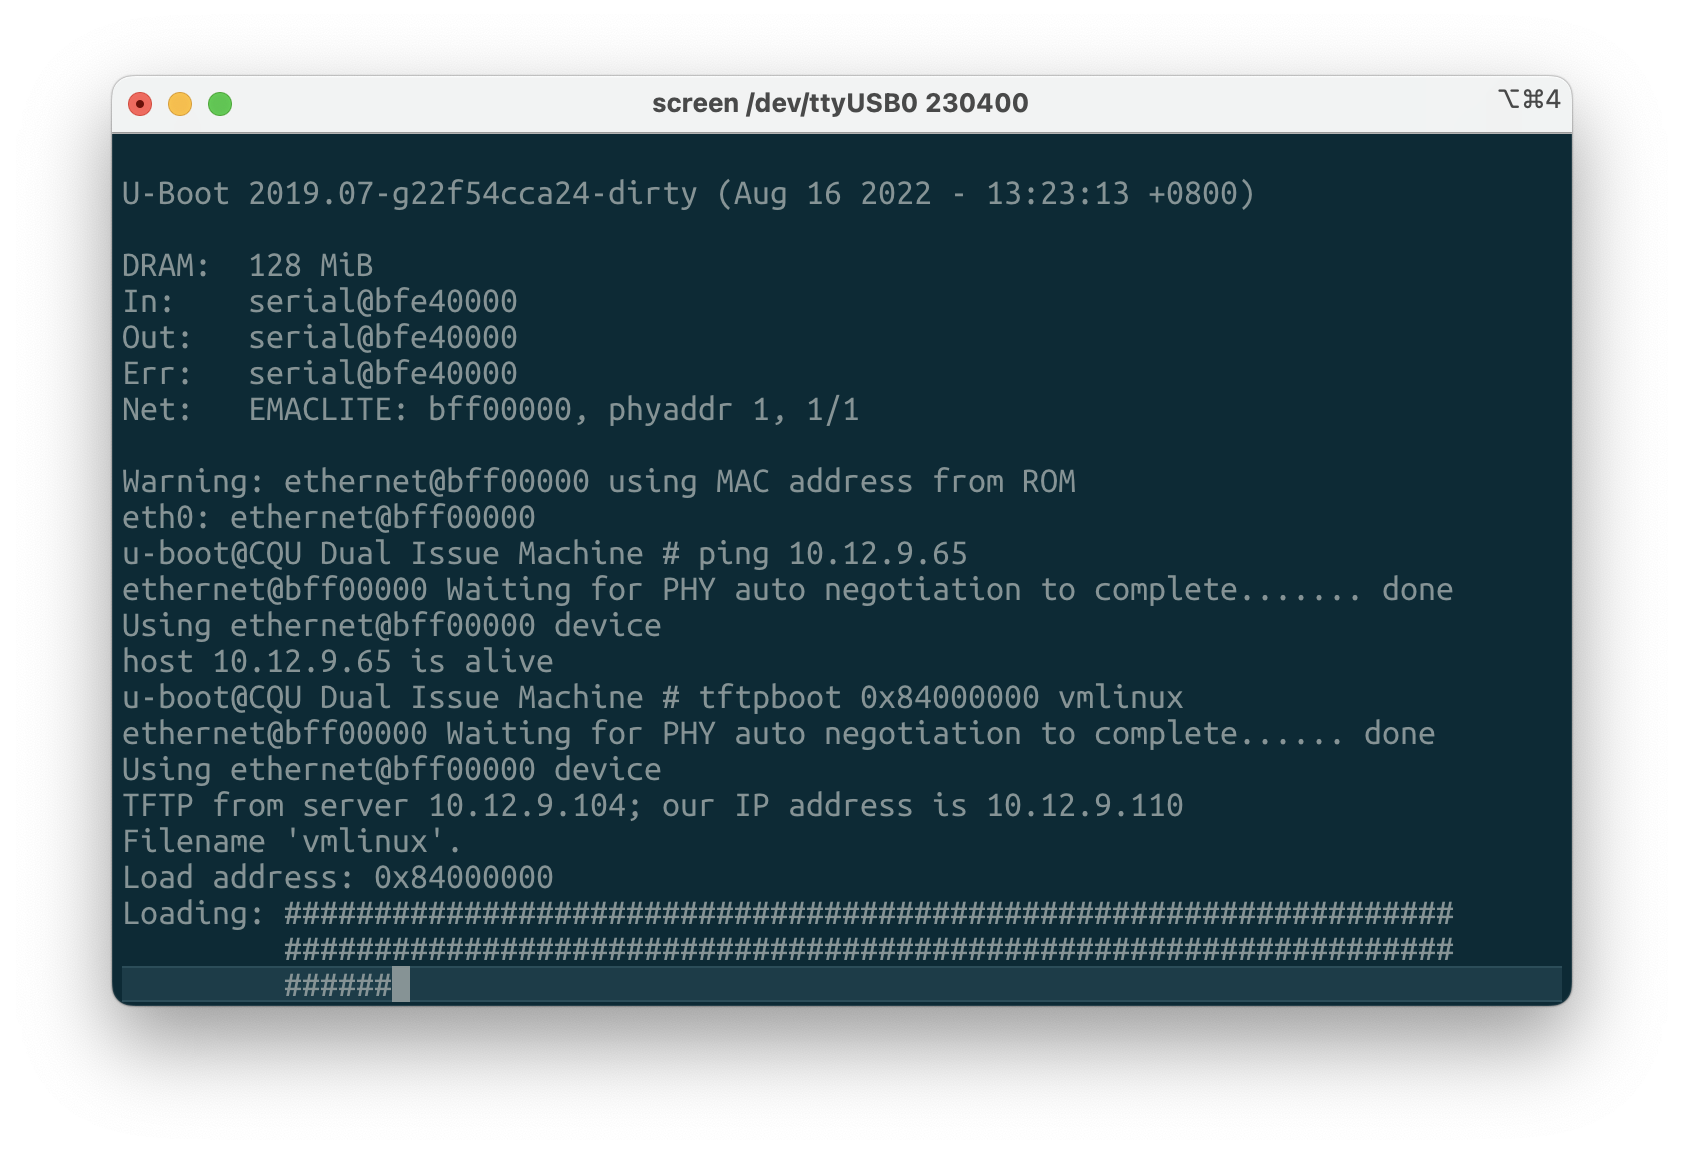
\includegraphics[width=\linewidth]{u-boot.png}
    \caption{U-Boot启动截图}
\end{figure}

\newpage

\section{uCore}

我们的处理器能够运行清华大学的教学操作系统uCore,并进入用户Shell执行程序。

\begin{figure}[htpb]
    \centering
    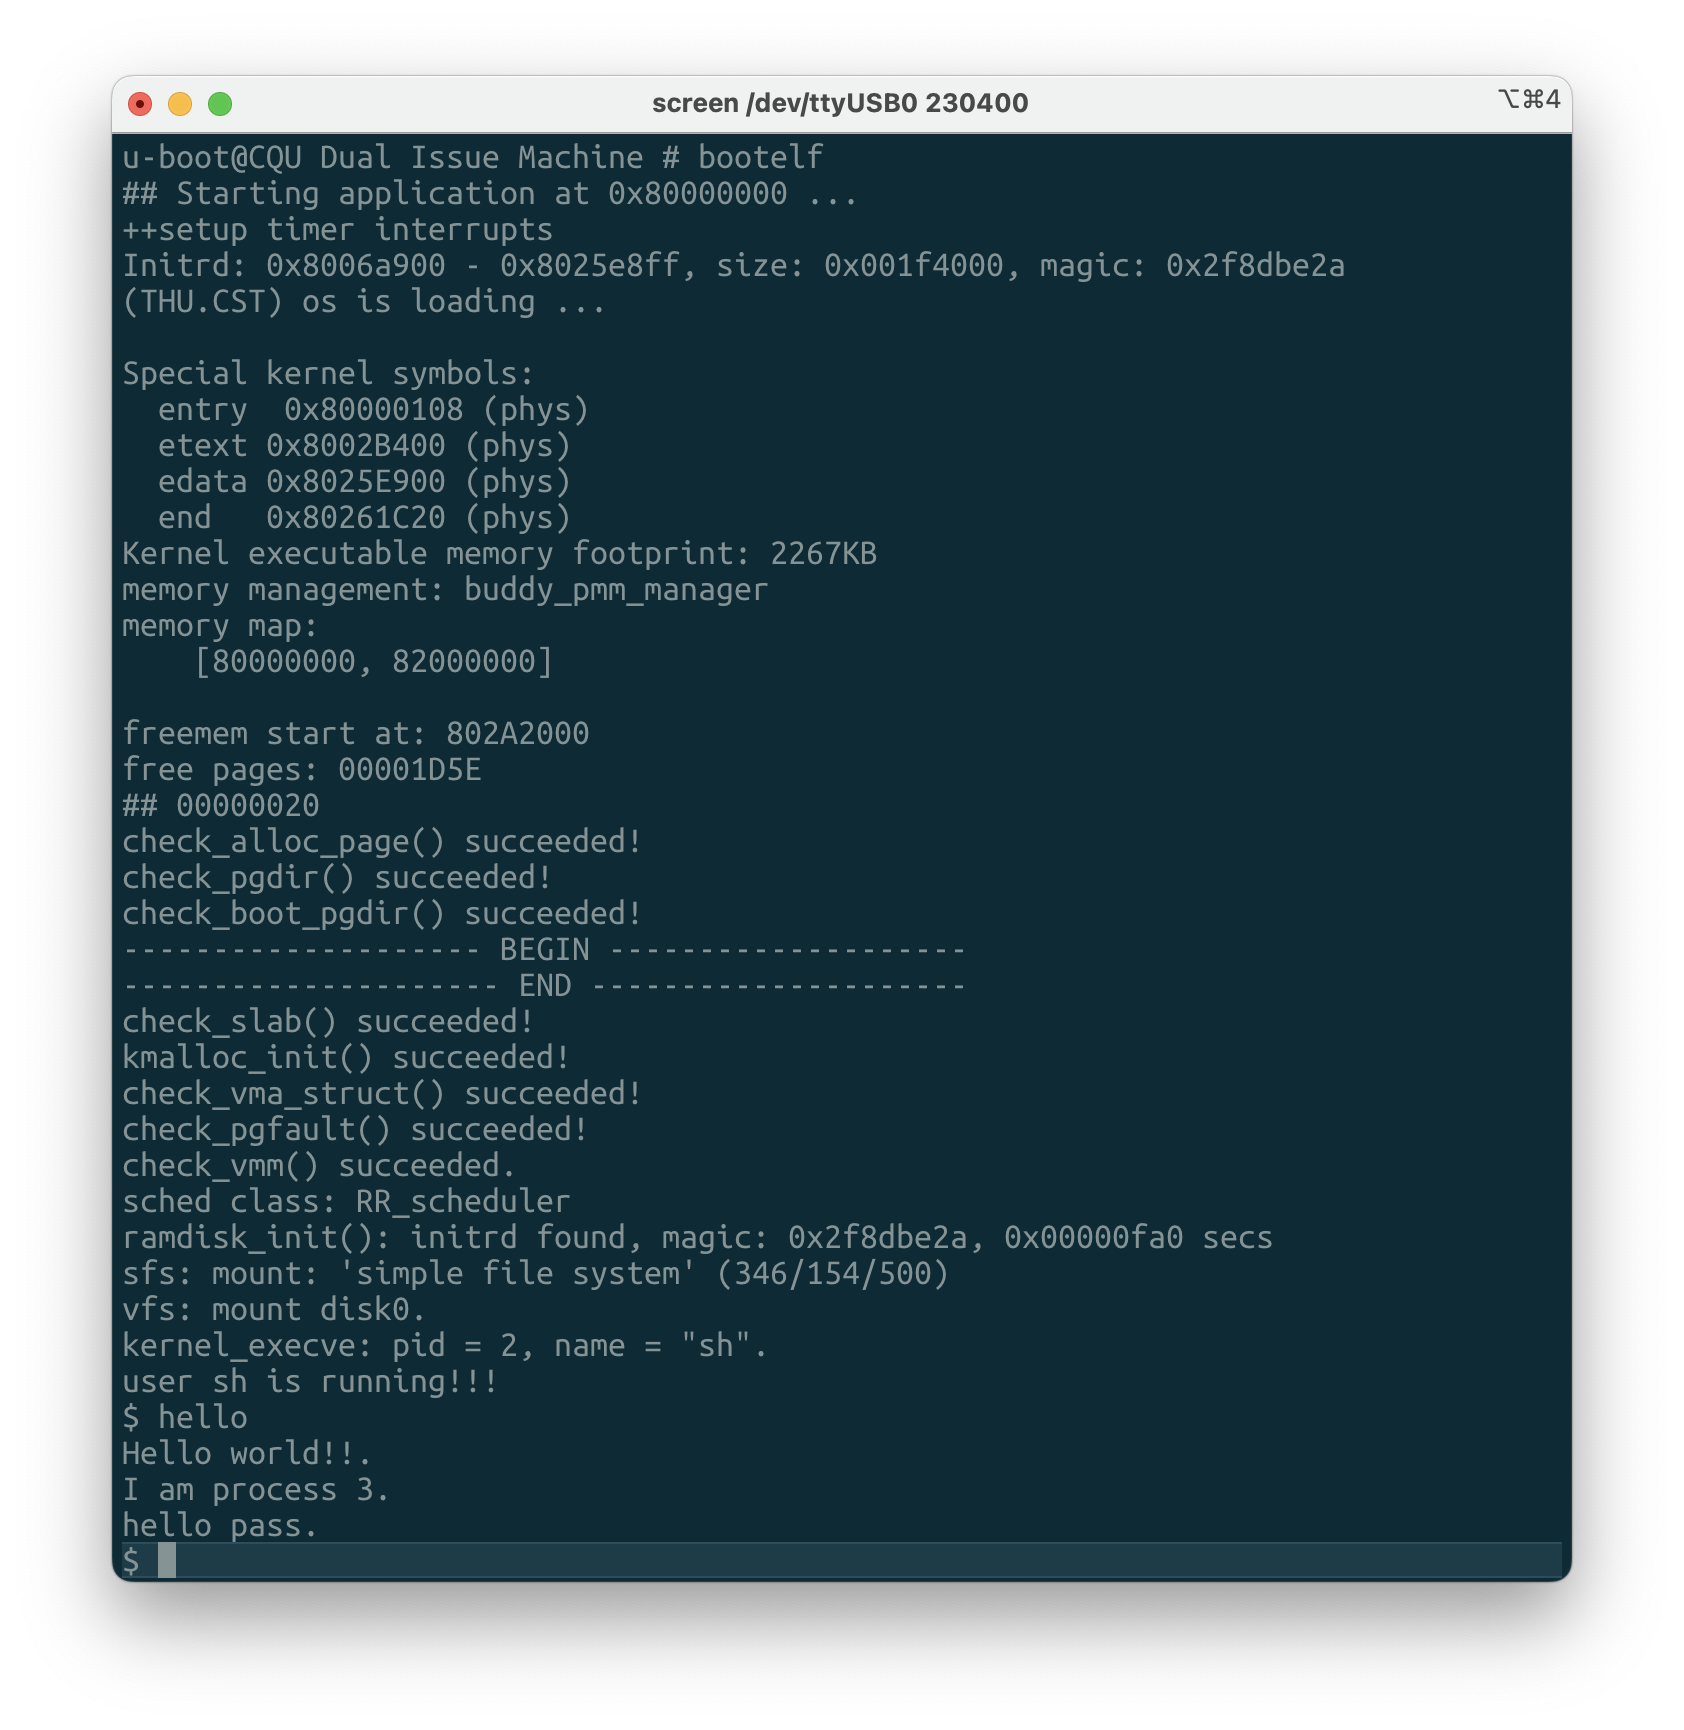
\includegraphics[width=\linewidth]{ucore.png}
    \caption{uCore运行截图}
    \label{img:ucore}
\end{figure}

\newpage

\section{Linux}

我们的处理器能够在编译器关闭Branch-Likely指令的情况下运行Linux v5.19,并自己编译了MIPS Release 1关闭浮点支持的Busybox,在Busybox中能够正常使用Shell。

在仿真SoC-Simulator与上板MegaSoC SoC上均测试成功,且能够使用SoC上的AXI Ethernet Lite IP核连接网络,能够使用wget访问www.nscscc.com网站并提取部分文字。

\begin{figure}[h]
    \centering
    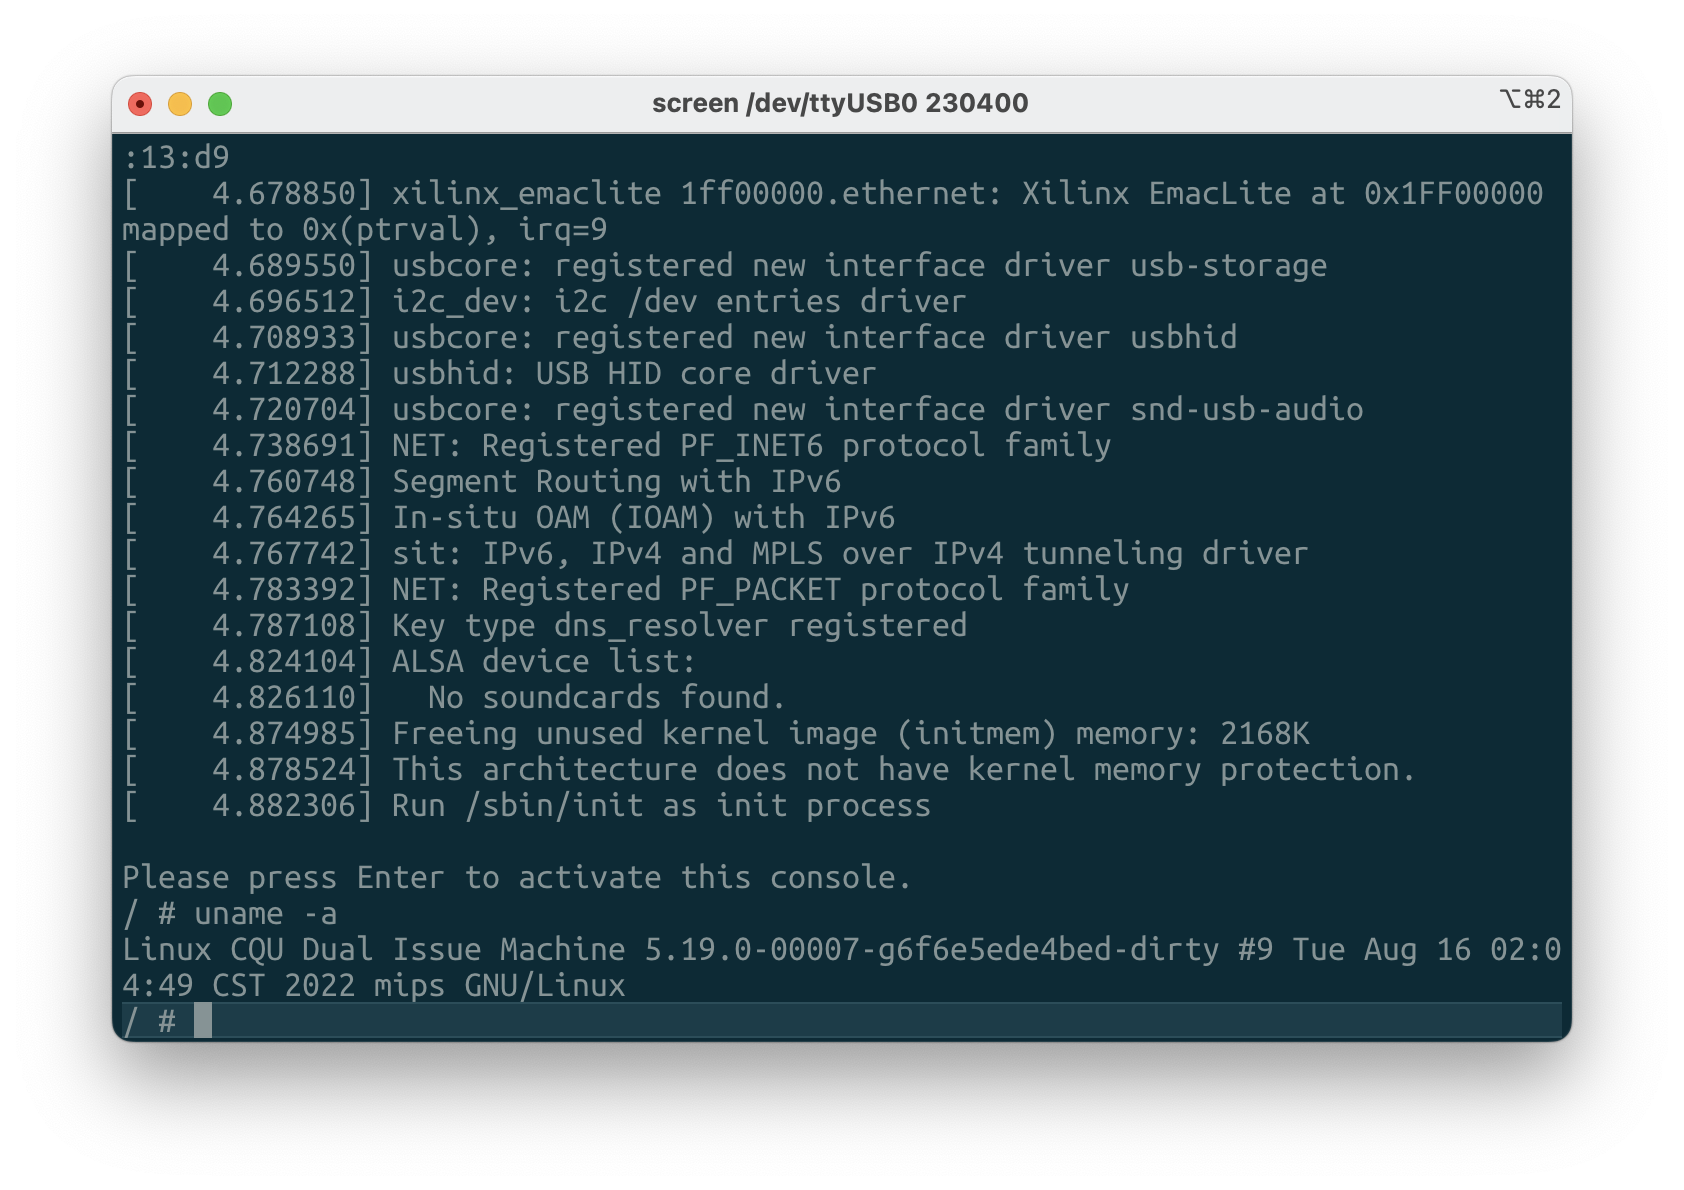
\includegraphics[width=\linewidth]{linux_boot.png}
    \caption{Linux启动截图}
    \label{img:linux_boot}
\end{figure}

\begin{figure}[h]
    \centering
    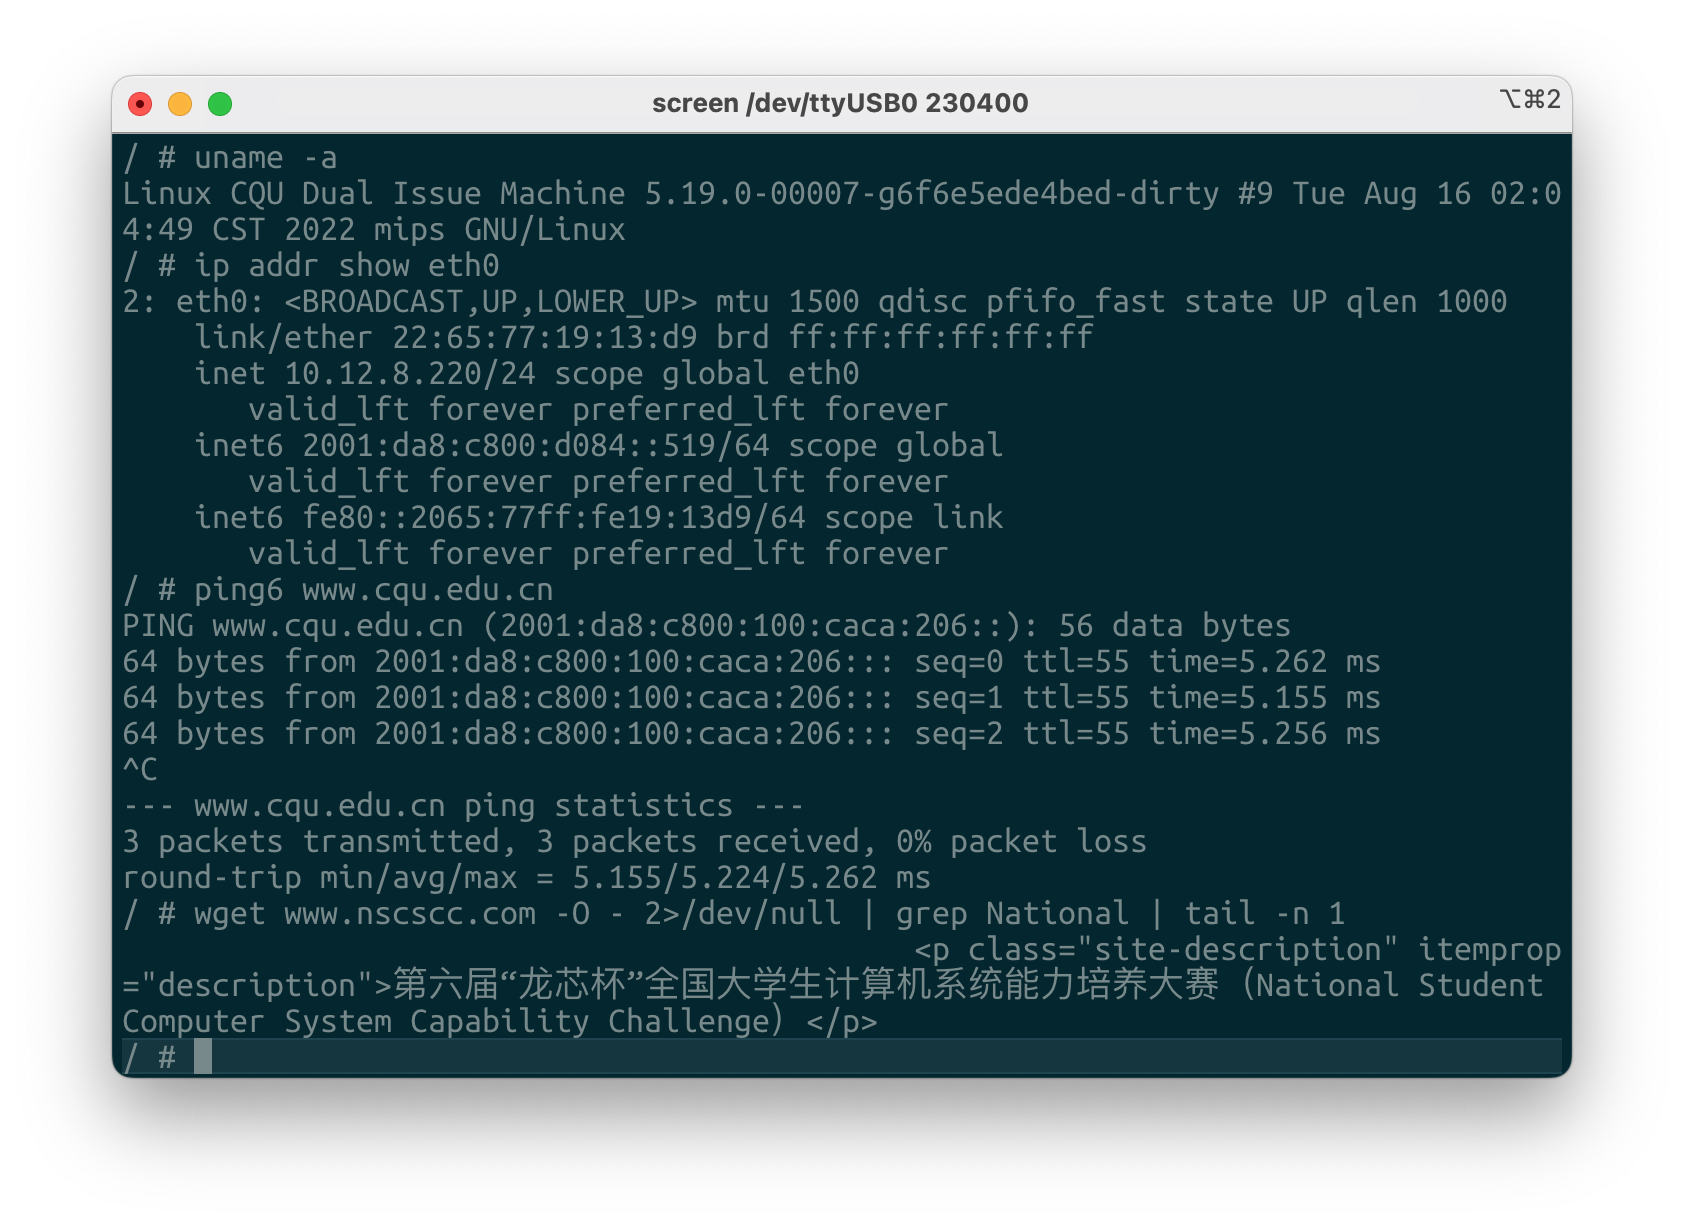
\includegraphics[width=\linewidth]{linux_nic_test.png}
    \caption{Linux上网截图}
    \label{img:linux_nic_test}
\end{figure}